\chapter{Planificación temporal}

\section{Estimación}

Se dispone de un tiempo limitado para la realización de este proyecto. Planificar correctamente en qué invertirlo antes de comenzar a trabajar es muy importante, ya que puede prevenir un malgasto innecesario del mismo en tareas que no aporten suficiente al avance del desarrollo, así como proporcionar guías de actuación ante cualquier imprevisto que pueda surgir durante el proceso.

El Trabajo de Fin de Grado proporciona al estudiante 12 créditos ECTS en el Grado. Según la normativa de la Universidad de Granada, un crédito ECTS equivale a entre 25 y 30 horas de trabajo, por lo que podemos estimar que se espera en el TFG una inversión de unas 300 horas como mínimo. El segundo cuatrimestre del curso académico 24/25 tiene una duración de 15 semanas, lo cual resultaría en unas 20 horas de trabajo por semana, o unas 4 horas al día.

Teniendo en cuenta los requisitos del proyecto, junto a este análisis realizado, se llega a la conclusión de que el modelo más compatible es un híbrido entre el modelo en cascada y la metodología ágil, siguiendo un desarrollo basado en funcionalidades.

En primer lugar, se planificará el trabajo como un proceso lineal, lo cual encaja con las limitaciones temporales, y permite dividir el proceso de desarrollo en dos grandes fases: una para el dispositivo, y otra para la interfaz, para no desaprovechar el tiempo desarrollando el aspecto visual de características que aun no existen. Después, se dividirá cada fase en distintas funcionalidades clave, que se irán implementando y probando una a una.

De esta forma, el avance en el proyecto es continuo, y se aprovechan las características ventajosas de ambos métodos. Por el lado del modelo en cascada, se evita invertir demasiado tiempo en la planificación de los distintos \textit{sprints}, de acuerdo al limitado tiempo disponible. En lo que a la metodología ágil respecta, se aprovecha la frecuente realización de pruebas, que asegura la calidad del producto final.

Representando las distintas fases del modelo en cascada, obtendríamos una planificación parecida a la siguiente:

\begin{figure}[ht]
	\centering
	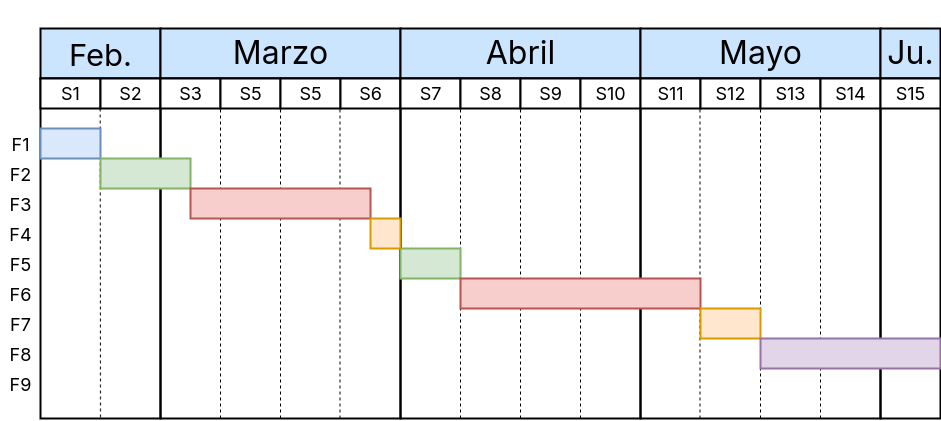
\includegraphics[width=\textwidth]{gantt.png}
	\caption{Diagrama de Gantt que muestra la organización de las distintas fases del proyecto a lo largo de las semanas.}
\end{figure}

\begin{itemize}
    \item Las fases de color azul representan la deficinición de los requisitos de cada parte del trabajo.
    \item Las verdes corresponden al tiempo de diseño.
    \item Las secciones rojas son las de desarrollo.
    \item Las fases de pruebas vienen señaladas en color naranja, siendo la segunda un poco más extensa para poder hacer pruebas de integración entre los dos sistemas.
    \item En morado está marcada la fase de documentación, que incluye tanto la del código como la generación de esta memoria.
\end{itemize}

Las tareas a realizar en cada fase serán detelladas más a fondo en sus capítulos correspondientes.

\section{Realidad}

En la práctica, el cumplimiento de esta planificación no ha sido posible, debido a haber tenido que compaginar el desarollo del proyecto con unas prácticas extracurriculares, y un posterior puesto de trabajo a tiempo completo.

Esto, junto a un pobre manejo del tiempo en algunas fases, ha provocado un avance más lento de lo esperado. Dichas desalineaciones han causado, a su vez, una mayor inversión de tiempo de la esperada en el proyecto, ascendiendo aproximadamente a unas 450 horas a lo largo de 5 meses.
